\subsection{Machine Code Translation}
\label{chap:qemu_translation}

As mentioned, QEMU at its core employs binary translation technology, allowing 
it to interpret and execute machine code compiled for one type of CPU on a 
completely different CPU. A typical binary translation converts the guest CPU's 
(also known as virtual CPU or vCPU) entire binary file into the host CPU's binary file 
using some method, and then executes the converted binary on the host CPU. 
However, this approach presents a significant problem, any modifications made to the 
guest program require, once again, a complete binary conversion. This wouldn't be 
a problem for small programs, but it is for larger ones. Longer conversion times may 
be acceptable for large guest programs if the conversion only needs to be done once. 
But, when frequent modifications to the guest program is need, like in embedded 
software development, this approach becomes impractical.

QEMU solves this problem by not implementing a traditional translation 
technology, instead use dynamic binary translation (DBT). This type of translation 
does not convert the entire vCPU program at once. it only converts the necessary parts 
of the program and executes them. For example, when booting a guest OS, only 
the parts required for booting are converted and executed. To be more specific, 
QEMU advances the program counter for the vCPU step by step, converting one 
vCPU instruction into one or more host CPU instructions and executing them, 
then advancing the program counter again, converting, executing, and repeating 
this process. With this method, there is no need to convert the parts that are 
not executed.

The inefficiency of translating the entire program binary from the vCPU is evident. 
However, translating and executing only one guest instruction at a time 
incurred a considerable time overhead. This is due to context management. 
QEMU is a regular program running on the host CPU, so to execute the instructions 
translated from the vCPU, it first needs to save the state of the host CPU's registers and 
memory context. Furthermore, once the translated instruction finishes executing, 
the saved state of the host CPU must be restored. Because of this inefficiency, 
DBT parses a short chunks of code, translates it, and caches the resulting sequence. 
This way, code is only translated as it is discovered and when possible, and branch 
instructions are configured to point to code that has already been translated and saved.

QEMU's DBT takes the named of the Tiny Code Generator (TCG), and the basic 
code fragments it analyzes are called Translation Blocks (TB). In the case of QEMU's 
TCG, the TBs are defined by using any instruction that changes the control flow of 
the program—jump or return instructions, interruptions or peripherals accesses—as 
boundaries\cite{QemuTCGOpsDevel}\cite{QemuTCGDirectBlockChaining}.

The translation performed by the TCG consists of two phases: converting the host 
code into a sequence of micro-operations and turning these micro-operations 
into executable code\cite{QemuTCGTechReport}. The figure \ref{fig:tcg} illustrates the general architecture and 
workflow of the TCG. Where the "Destination Machine Code" corresponds to a TB, the 
XXX portion of the diagram represents the TCG, and the last block represents the 
"Host Machine Code".

\begin{figure}[H]
    \centering
%    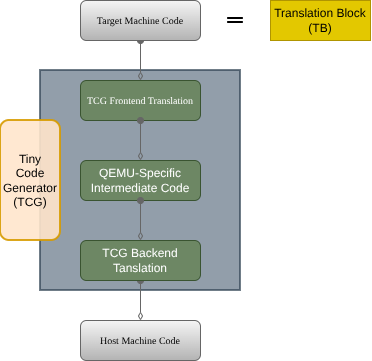
\includegraphics[width=0.5\textwidth]{Resources/Draw/TCG.png}
    \caption{Tiny Code Generator}
    \label{fig:tcg}
\end{figure}

In the first phase, the TCG's frontend section decomposed each guest instruction 
from the corresponding TB into equivalent sequences of QEMU-specific intermediate 
representations (IRs), called micro-operations. Conceptually, these micro-operations 
are like an assembly language designed specifically for QEMU's compilation infrastructure.

In the second phase, the TCG's back-end section converts this intermediate 
representation into native host machine code, which is then directly executable on 
the host processor\cite{QemuTCGFrontendOps}\cite{QemuTCGBackendOps}. The TCG maintains a dictionary of micro-operations. 
This dictionary contains a mapping between micro-operations and the equivalent 
sequences of host architecture binary code. This binary code performs the task of 
the corresponding micro-operation when run on the host processor. The TCG cycles 
through each micro-operation contained in the translation block and emits the 
corresponding sequence of host machine instructions by using the dictionary. 
The result is a block of host machine code that performs the same operations as the 
guest machine code\cite{QemuTCGTechReport}.

The QEMU developers' decision to separate front-end and back-end translation 
was a wise one, as it offers significant advantages for QEMU's scalability. Thanks 
to this decision, to support a new host CPU architecture, developers only need to 
implement a new front-end translator, while the back-end translation logic remains 
unchanged. Conversely, supporting QEMU on a new host architecture only requires 
back-end development, without affecting compatibility with that architecture. This 
modularity is the primary reason for QEMU's scalability across various hardware 
platforms and CPU architectures.
